\chapter{\twor}
\label{two}
\begin{wrapfigure}{l}{0.05\textwidth}

\includegraphics[width=\linewidth]{img/common/logo.png}
\label{fig:wrapfig2}
\end{wrapfigure}

\paragraph{What is it?} The \textit{\twor} sample is a malicious Android application masquerading as a plug-in for a transportation app series developed by a South Korean developer. The legitimate series provides bus-related information, such as bus stop locations and arrival times, which makes the repackaged sample appear trustworthy at first glance. The package name \texttt{lmh.android.gjbus} and the internal name \texttt{gjbus} are consistent with a localised variant of the same Malbus family, targeting the Gwangju metropolitan area.

\section{VirusTotal}
\begin{figure}[htbp]
        \centering
        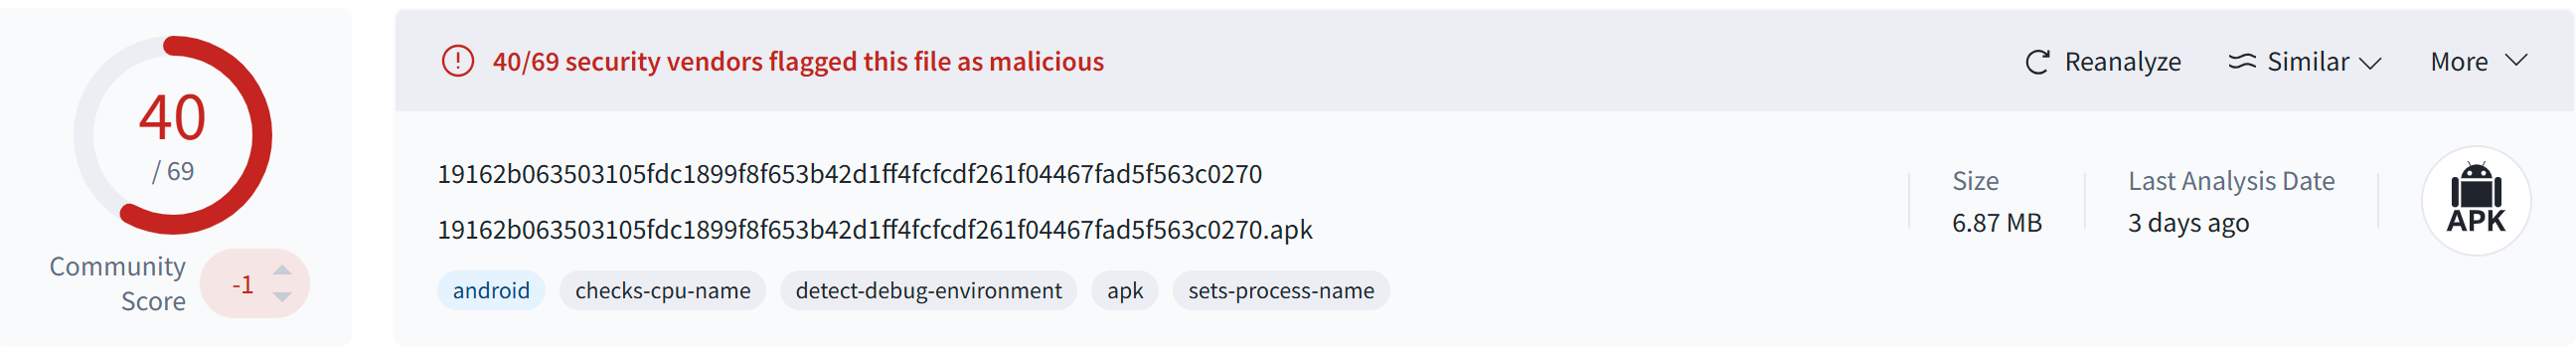
\includegraphics[width=\textwidth]{img/apk_2/virustotal_2_summary.png}
        \caption{VirusTotal Summary for \twor}
        \label{fig:virustotal_2_summary}
\end{figure}

\subsection{Detection}
The antimalware analysis performed with VirusTotal shows that \texttt{40/75} security vendors flagged the file as malicious, while \texttt{28/75} vendors classified it as a secure file, \texttt{1/75} reported a failure error, and \texttt{6/75} vendors reported an \textit{Unable to process file type} error.
Most engines identify the sample as a generic Android trojan, and some of them further classify it as a downloader-family specimen. A few vendors instead label it only as generic Android malware, without specifying a precise family.
It is also noteworthy that some well-known vendors, including Microsoft Defender, McAfee, and Malwarebytes, did not identify the file as malicious.

VirusTotal assigns the sample a reputation score of \texttt{-2} and a suggested threat label of \texttt{trojan.andr/apkdownloader}. The popular threat classification aggregated across all detecting engines identifies ``trojan'' as the dominant category (17 engines), followed by ``downloader'' (4 engines) and ``dropper'' (1 engine). Notably, the engine Tencent identifies the sample under the specific name \texttt{a.privacy.MalBuslmh}, a designation that directly references the APK package namespace \texttt{lmh}, confirming that this specific sample is known to the threat intelligence community.

\begin{figure}[h]
        \centering
            \begin{subfigure}[t]{0.48\linewidth}
        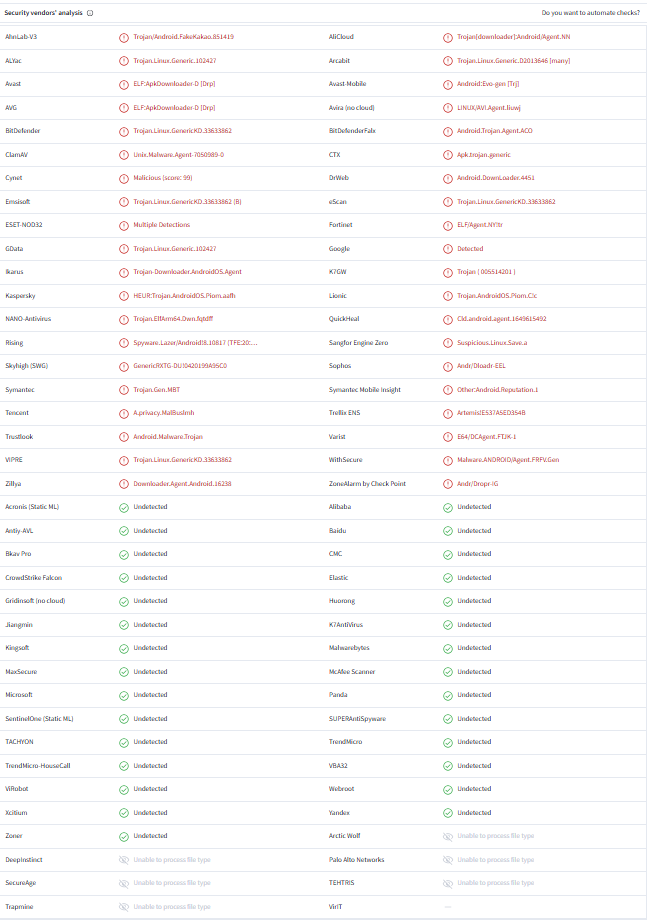
\includegraphics[width=0.8\linewidth]{img/apk_2/virustotal_2_detection_complete.png}
        \caption{VirusTotal Detection for \twor}
        \label{fig:virustotal_2_detections}
        \end{subfigure}
    \hfill
    \begin{subfigure}[t]{0.48\linewidth}
            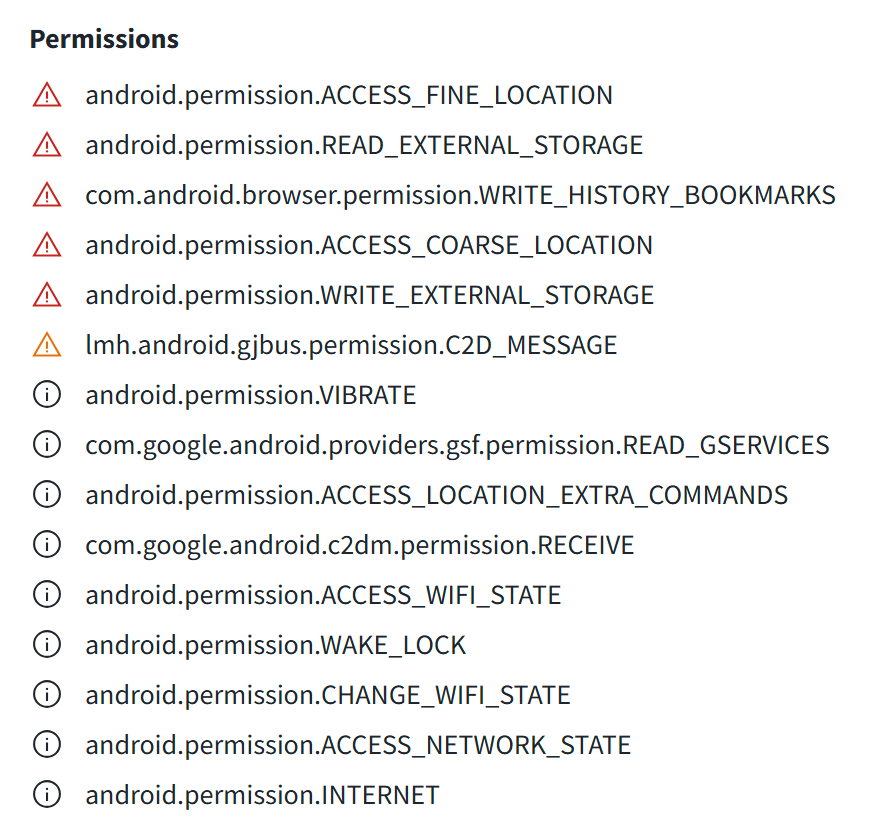
\includegraphics[width=0.8\linewidth]{img/apk_2/virustotal_second_permissions.png}
        \caption{Android Permissions of \twor}
        \label{fig:virustotal_2_permissions}
        \end{subfigure}
\end{figure}

\subsection{Details}
Here is a detailed analysis of the permissions which are required by the APK, declared in the Manifest file (Fig.\ \ref{fig:manifest_second}):
\begin{enumerate}
\item \textbf{android.permission.ACCESS\_FINE\_LOCATION} $\rightarrow$ Allows the precise location of the device (GPS, mobile networks, Wi-Fi).
\item \textbf{android.permission.ACCESS\_COARSE\_LOCATION} $\rightarrow$ Provides approximate location (based on cellular towers and Wi-Fi).
\item \textbf{android.permission.ACCESS\_LOCATION\_EXTRA\_COMMANDS} $\rightarrow$ Allows additional commands to be sent to the location provider (rarely used in legitimate apps).
\item \textbf{android.permission.READ\_EXTERNAL\_STORAGE} $\rightarrow$ Allows reading files and data saved on external memory (photos, documents, downloads).
\item \textbf{android.permission.WRITE\_EXTERNAL\_STORAGE} $\rightarrow$ Allows you to create or edit files on external storage.
\item \textbf{android.permission.INTERNET} $\rightarrow$ Enables any network connection (HTTP, sockets, DNS).
\item \textbf{android.permission.ACCESS\_NETWORK\_STATE} $\rightarrow$ Reads the status of network connections (Wi-Fi, mobile data).
\item \textbf{android.permission.ACCESS\_WIFI\_STATE} $\rightarrow$ Gets information about Wi-Fi networks (SSID, BSSID, status).
\item \textbf{android.permission.CHANGE\_WIFI\_STATE} $\rightarrow$ Changes Wi-Fi status (enable/disable, connects to networks).
\item \textbf{android.permission.WAKE\_LOCK} $\rightarrow$ Prevents the device from entering sleep mode.
\item \textbf{android.permission.VIBRATE} $\rightarrow$ Controls the vibration engine.
\item \textbf{lmh.android.gjbus.permission.C2D\_MESSAGE} $\rightarrow$ Enables reception of cloud-to-device messages (C2DM/GCM/FCM).
\item \textbf{com.google.android.c2dm.permission.RECEIVE} $\rightarrow$ Allows push notifications via Google Cloud Messaging (GCM/FCM).
\end{enumerate}

In addition to the permission analysis, VirusTotal assigns several behavioural and structural tags to the file: \texttt{sets-process-name}, \texttt{obfuscated}, \texttt{reflection}, \texttt{checks-cpu-name}, \texttt{telephony}, \texttt{detect-debug-environment}, \texttt{checks-gps}, \texttt{android}, and \texttt{apk}. The tags \texttt{obfuscated} and \texttt{reflection} are consistent with the use of Java Reflection observed during static analysis. The tags \texttt{detect-debug-environment}, \texttt{checks-cpu-name}, and \texttt{sets-process-name} are explicit anti-analysis and VM evasion indicators, consistent with the same pattern observed in the third sample. The \texttt{telephony} tag further indicates interaction with device communication APIs, which is not expected for a bus-information application.

\subsection{Relations}

\begin{figure}[h]
        \centering
        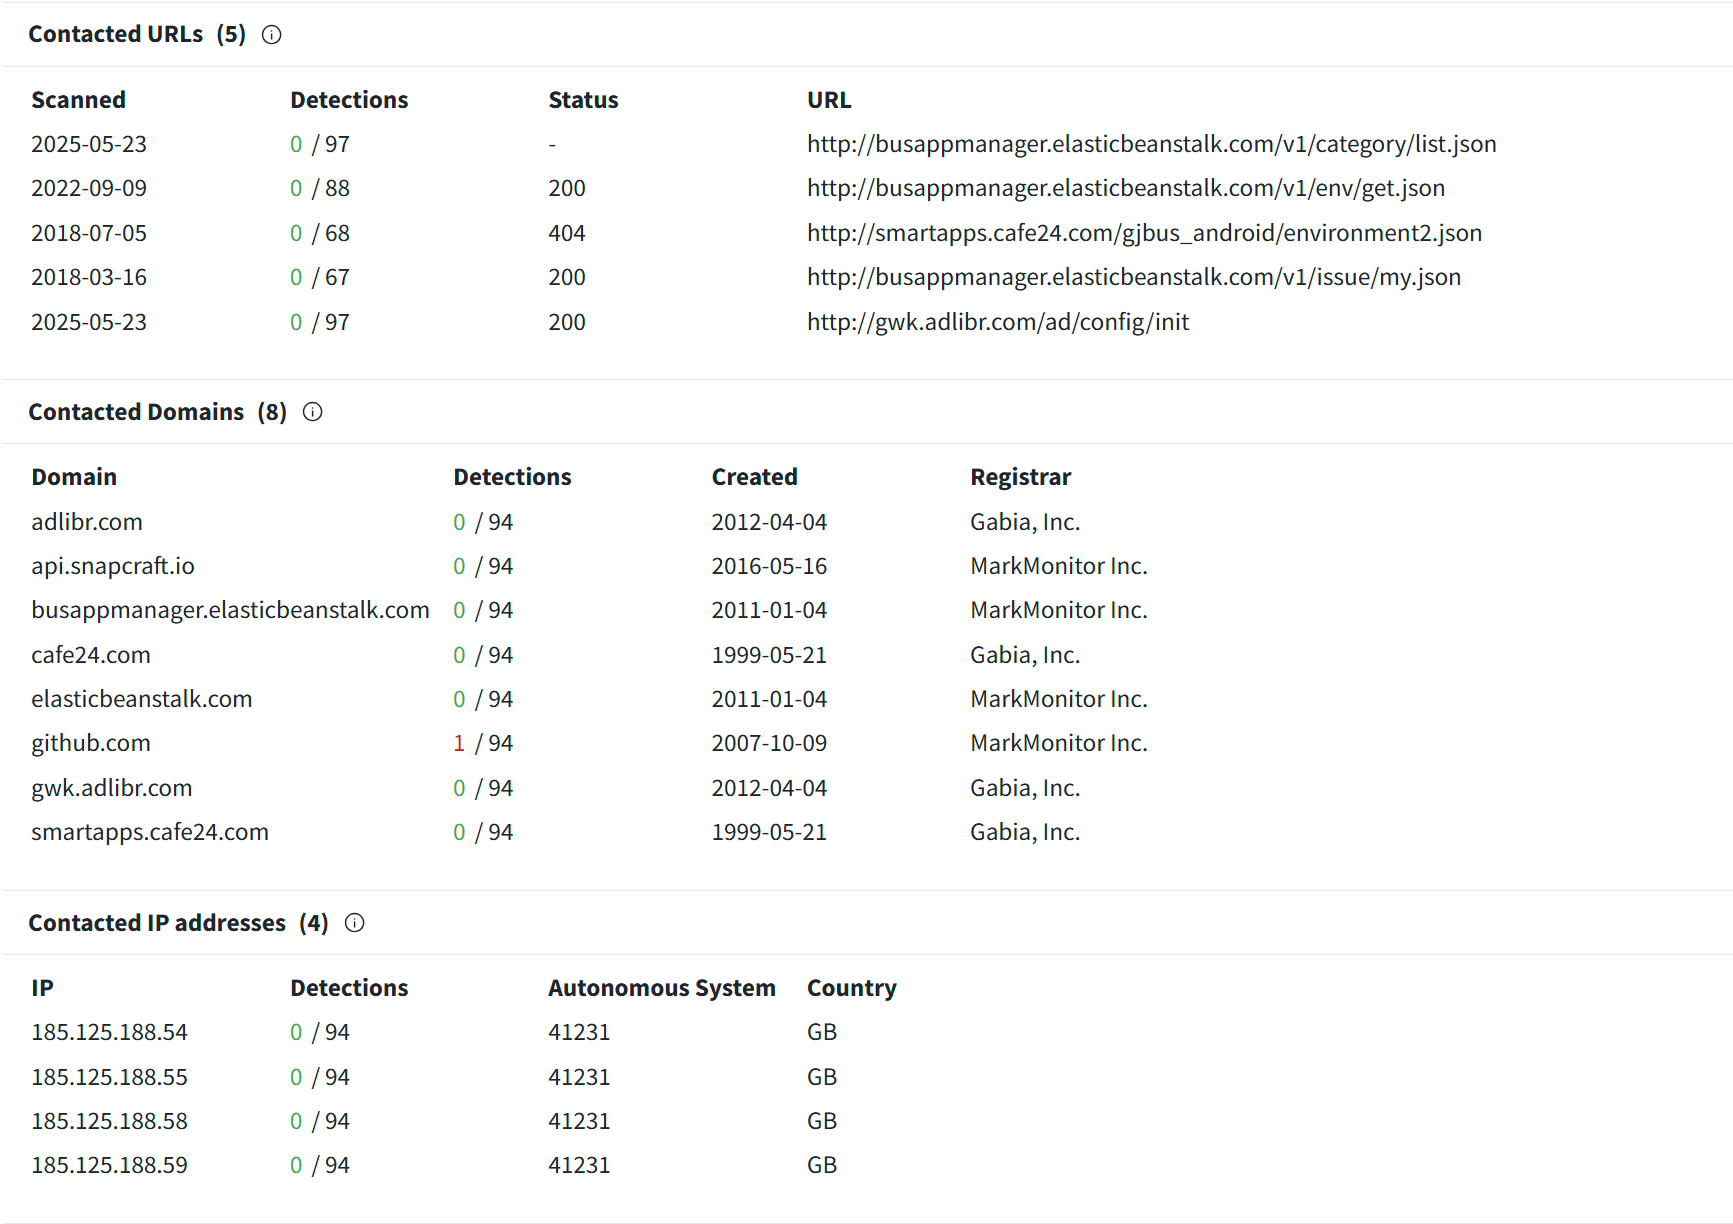
\includegraphics[width=\textwidth]{img/apk_2/second_relations.png}
        \caption{VirusTotal Relations for \twor}
        \label{fig:virustotal_2_relations}
\end{figure}

VirusTotal, as shown in Fig.\ \ref{fig:virustotal_2_relations}, reports multiple contacted URLs, domains, and IP addresses associated with the APK. The contacted URLs are all served over plain HTTP:

\begin{itemize}
    \item \texttt{http://busappmanager.elasticbeanstalk.com/v1/category/list.json}
    \item \texttt{http://busappmanager.elasticbeanstalk.com/v1/env/get.json}
    \item \texttt{http://busappmanager.elasticbeanstalk.com/v1/issue/my.json}
    \item \texttt{http://smartapps.cafe24.com/gjbus\_android/environment2.json}
    \item \texttt{http://gwk.adlibr.com/ad/config/init}
\end{itemize}

The first three URLs are hosted on AWS Elastic Beanstalk and appear to retrieve the app category list, runtime environment configuration, and remote issue data from a centralised backend. This mechanism is consistent with dropper-like behaviour, as it allows the app to modify its functionality without requiring a new APK release. The fourth URL (\texttt{smartapps.cafe24.com}) retrieves a configuration file specific to this \texttt{gjbus} variant, using a path (\texttt{/gjbus\_android/environment2.json}) that distinguishes it from the other regional Malbus samples. The domain \texttt{gwk.adlibr.com/ad/config/init} serves the advertising configuration; it responds only to POST requests, otherwise returning \texttt{\{"result":4003,"message":"key\_media\_key"\}}.

VirusTotal also records several alternative names under which the sample has been submitted across its 354 total submissions: \texttt{bus.apk}, \texttt{malbus.apk}, \texttt{lmh.android.gjbus.apk}, \texttt{00081.apk}, and others. The variety of filenames under which the same hash appears suggests that the sample has been distributed or repackaged under different labels, which is consistent with trojanised application behaviour.

\subsection{Behavior}

The behaviour tab indicates that the APK accesses file-related resources, builds JSON objects from filenames and absolute paths, reads data through buffer streams, and opens files from absolute paths.
It also shows the use of reflection or control-based execution to start another application from the current one, which may indicate indirect execution of external components. In addition, the sample interacts with advertising and analytics libraries, schedules recording tasks, and reads files from the assets directory.

Notably, this variant carries explicit \textbf{anti-analysis and VM evasion} indicators consistent with the third Malbus sample. VirusTotal tags the APK with \texttt{detect-debug-environment}, indicating that the application actively probes for debugger and sandbox contexts at runtime. The tag \texttt{checks-cpu-name} reveals hardware fingerprinting consistent with virtual machine detection, and \texttt{sets-process-name} indicates process name manipulation to obfuscate the running process from monitoring tools.

Overall, the observed behaviour is more complex than that of a simple bus-information client and is compatible with a repackaged application that supports file-system interaction, dynamically driven actions, and active evasion of analysis environments.
Additionally, as observed in the first Malbus sample, a crowdsourced YARA rule match was recorded for this sample: the IcedID structural rule from the CAPEv2 repository matched the binary. As discussed in Chapter~\ref{one}, this does not imply family membership but confirms structural similarity with known dropper and loader architectures.
\section{Static Analysis}
The Java source code was decompiled using JD-GUI / Bytecodeviewer and inspected manually to identify classes and methods of interest.
Static analysis shows that the application combines legitimate bus-related functionality with advertising SDKs, remote configuration mechanisms, native code, and update-like behaviour. This indicates that the APK is not limited to its declared purpose, but may also support conditional execution and payload delivery at runtime.

\subsection{MainActivity.java}
\begin{itemize}
    \item Inherits from \texttt{BaseMainActivity}.
    \item Calls \texttt{getTabView(BaseTabFragmentActivity.MainTabs.BUSTRANS).setVisibility(8)} to hide a UI tab.
    \item Provides ad-network keys through \texttt{getAdvertiseKey(...)}.
    \item Retrieves configuration through \texttt{getEnvironmentProperties(...)}.
\end{itemize}

This combination suggests that the visible interface is at least partially controlled at runtime. In particular, the hiding of a UI tab and the retrieval of external configuration parameters imply that the application may adapt its behaviour according to remotely supplied values.
The use of multiple advertising providers, including AdMob, Facebook, and AdLib, further confirms the presence of monetization-oriented logic.

\subsection{BaseMainActivity.java}
\begin{itemize}
    \item Acts as the central initialization hub.
    \item Loads the native library with \texttt{System.loadLibrary("Audio3.0")}.
    \item Declares and invokes the native methods \texttt{startUpdate()} and \texttt{updateApplication()}.
    \item Requests the runtime permissions:
    \begin{itemize}
        \item \texttt{READ\_EXTERNAL\_STORAGE}
        \item \texttt{WRITE\_EXTERNAL\_STORAGE}
        \item \texttt{REQUEST\_INSTALL\_PACKAGES}
    \end{itemize}
    \item Loads remote app environment data, including a URL, a database version, and a remote download URL.
\end{itemize}

This class is the most relevant part of the static analysis. The presence of a native library, together with methods related to update handling and the request for \texttt{REQUEST\_INSTALL\_PACKAGES}, is consistent with dropper-like behaviour. In addition, the remote environment loading mechanism allows the application to modify its behaviour without requiring a new release.

\subsection{EnvConstant.java}
The \texttt{EnvConstant} class defines several hardcoded advertising and analytics keys. MobSF confirmed the extraction of hardcoded secrets including \texttt{adpostkey}, \texttt{adlibkey}, and hash keys embedded directly in the source code.

\begin{lstlisting}[language=Java]
public static final String ADAM_KEY = "3034Z1OT1385cf1db09";
public static final String ADLIB_KEY = "590ea88a0cf2843c93807ed9";
public static final String ADMOB_UNITID = "ca-app-pub-0388605861855854/7499990747";
public static final String FACEBOOK = "627046304133735685335228304842";
public static final String GA_TRACKER_ID = "UA-56668425-6";
\end{lstlisting}

These constants confirm the integration of multiple ad SDKs and tracking frameworks. Although no endpoint URLs are directly visible in this file, the constants are consistent with the remote-configuration logic observed in the main activity.

\subsection{BusApiWeb.java}
\texttt{BusApiWeb} performs network requests to bus-related endpoints over plain HTTP. It uses Volley for networking, parses HTML responses instead of JSON, and relays information through listeners.
\begin{itemize}
    \item Makes calls to \texttt{http://bus.changwon.go.kr/busInfo/busInfoDetail.jsp} and \texttt{http://bus.changwon.go.kr/busInfo/mapLayer.jsp}.
    \item Uses Volley for networking.
    \item Parses HTML responses instead of JSON.
    \item Relays information through listeners.
\end{itemize}
The main issue in this component is the exclusive use of HTTP. Since the communication is not protected by TLS, bus-stop identifiers and route data travel in plaintext and can be intercepted or modified in transit, creating a clear man-in-the-middle risk.

\subsection{AndroidManifest.xml}

\begin{figure}[h]
        \centering
        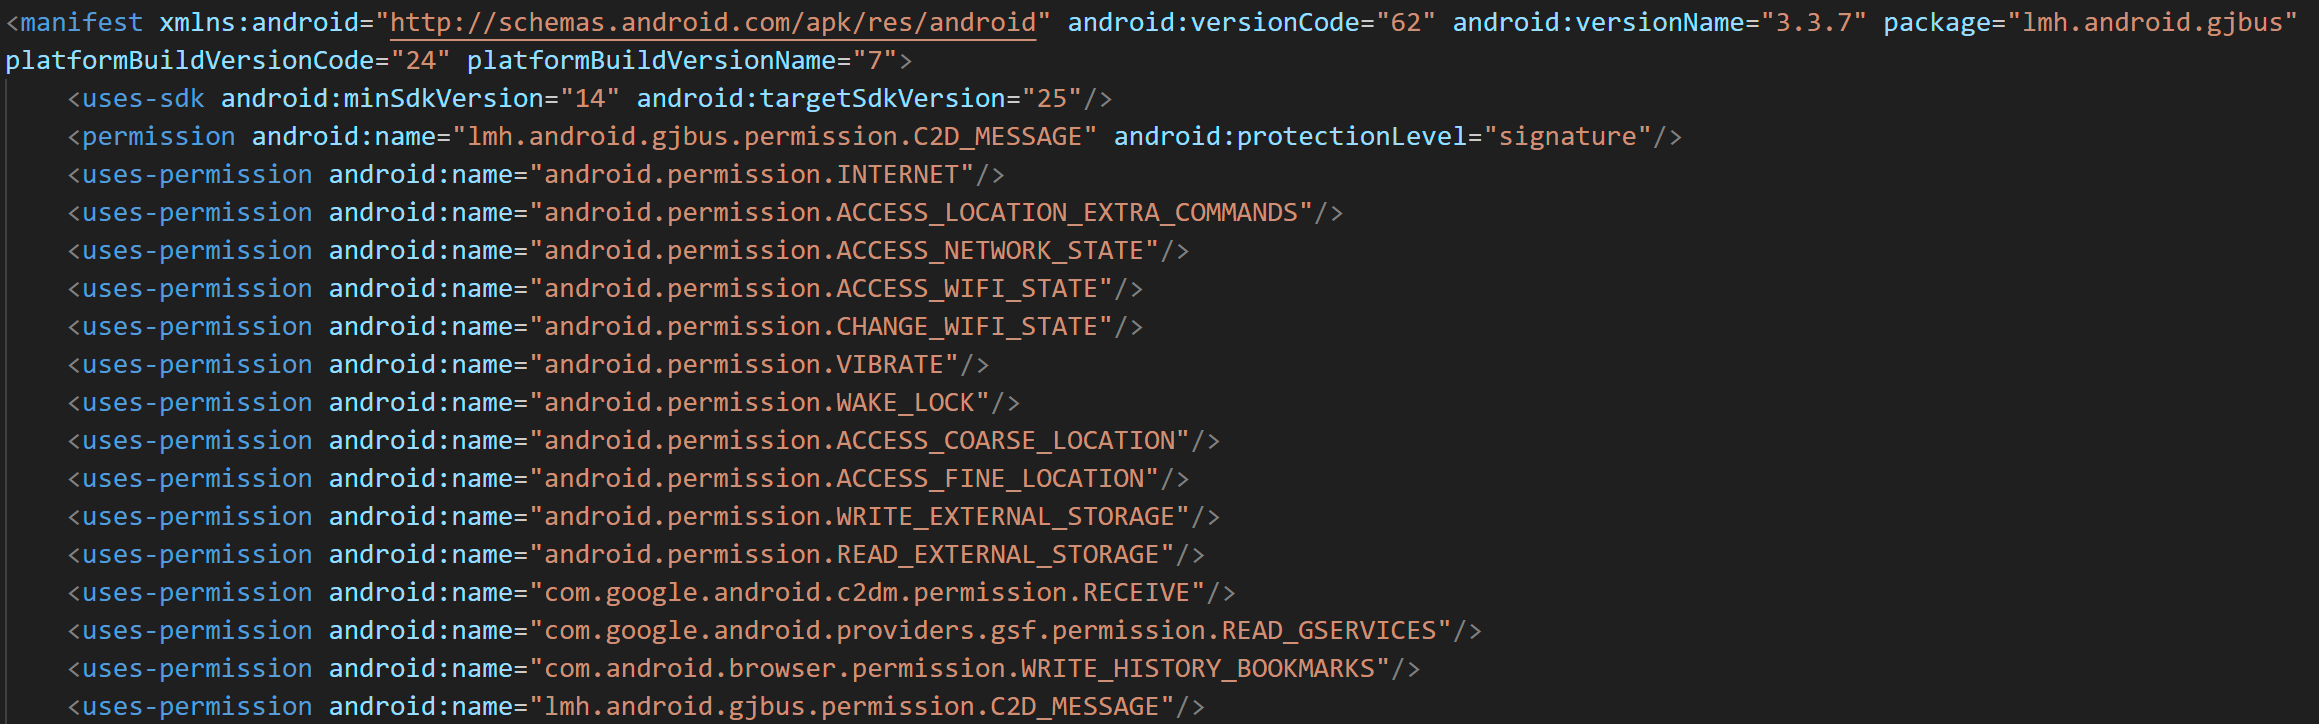
\includegraphics[width=\textwidth]{img/apk_2/manifest_second.png}
        \caption{AndroidManifest of \twor}
        \label{fig:manifest_second}
\end{figure}
\begin{itemize}
    \item Declares the following permissions:
    \begin{itemize}
        \item \texttt{INTERNET}, \texttt{ACCESS\_FINE\_LOCATION}, \texttt{ACCESS\_COARSE\_LOCATION}
        \item \texttt{READ\_EXTERNAL\_STORAGE}, \texttt{WRITE\_EXTERNAL\_STORAGE}
        \item \texttt{REQUEST\_INSTALL\_PACKAGES}
    \end{itemize}
    \item Declares multiple ad and analytics activities:
    \begin{itemize}
        \item AdLib, AdMob, Facebook, AdFit (Kakao)
    \end{itemize}
    \item Includes GCM and Firebase messaging support.
    \item Declares the custom service \texttt{lmh.android.gjbus.GCMIntentService}.
\end{itemize}
The manifest confirms that the application can receive background messages and interact with external services. In particular, the presence of \texttt{REQUEST\_INSTALL\_PACKAGES} is significant because, if granted, it may allow silent installation of additional APKs. Combined with GCM/Firebase messaging, this suggests the possibility of remote triggering of behaviour.

\subsection{AppInfoActivity.java}
\begin{itemize}
    \item Displays a public bus-related URL for the Gwangju city service.
    \item Serves to legitimize the app.
    \item Contains no interaction logic.
\end{itemize}
This activity appears to be mainly cosmetic. Its role seems to be presenting the application as a legitimate transportation service, even though the rest of the static analysis reveals a much more complex and suspicious architecture.

\section{Summary}

\begin{longtable}{|p{0.45\textwidth}|p{0.45\textwidth}|}
\hline
\textbf{Suspicious Pattern} & \textbf{Explanation} \\
\hline
Multiple ad SDKs & Monetization through aggressive advertising and possible ad fraud. \\
\hline
Native libraries (JNI) & Executes code not visible to standard Java analysis tools. \\
\hline
\texttt{REQUEST\_INSTALL\_PACKAGES} & Suggests dropper-like behaviour and possible APK installation without market interaction. \\
\hline
Unencrypted HTTP endpoints & Data can be intercepted or modified through MITM attacks. \\
\hline
Dynamic configuration via \texttt{getEnvironmentProperties(...)} & The app can change behaviour based on remote values. \\
\hline
Fragment and tab visibility manipulation & Suggests conditional or delayed functionality and may hide behaviour from users and analysts. \\
\hline
VT behavioural tags (\texttt{obfuscated}, \texttt{telephony}, \texttt{checks-gps}) & Confirm runtime obfuscation, device tracking via GPS, and telephony API interaction beyond the declared app purpose. \\
\hline
Anti-analysis \& VM evasion (\texttt{detect-debug-environment}, \texttt{checks-cpu-name}, \texttt{sets-process-name}) & The app actively probes for debuggers and sandboxes and manipulates its process name to evade monitoring tools; consistent with the third Malbus sample. \\
\hline
Alternative submission names (354 submissions) & \texttt{bus.apk}, \texttt{malbus.apk}, \texttt{lmh.android.gjbus.apk} confirm distribution under multiple filenames, consistent with trojanised repackaging. \\
\hline
\end{longtable}

\section{MobSF}

\begin{figure}[h]
    \centering
    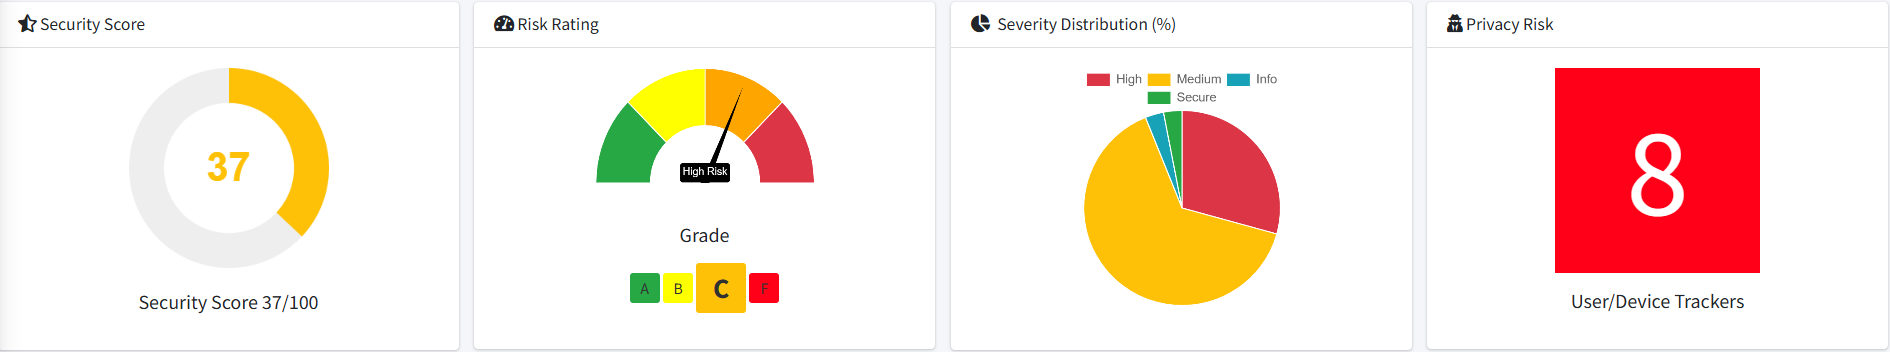
\includegraphics[width=\linewidth]{img/apk_2/mobsf_two_scorecard.png}
    \caption{MobSF Scorecard \twor}
    \label{fig:mobsf_scorecard_two}
\end{figure}
MobSF assigned a security score of 37/100 (Grade C, HIGH RISK) to this APK, confirming that the application exposes a broad attack surface.
In particular, the scorecard shows problems related to signature schemes, outdated Android compatibility, exported components, insecure storage, and the presence of multiple privacy trackers.

\subsection{Certificate Analysis}
During the MobSF analysis, one unique certificate was found. The binary is signed with the \texttt{v1} signature scheme only, while \texttt{v2}, \texttt{v3}, and \texttt{v4} are absent. The certificate uses \texttt{SHA1withRSA}, with subject and issuer both identified as \texttt{C=ko, L=Gwangju, CN=Myoung-Hun Lee}. The validity interval spans from 2011-05-09 to 2061-04-26, and the reported hash algorithm is SHA-1. This signing configuration is weak from a security perspective because it relies on legacy mechanisms associated with known cryptographic and platform-level weaknesses, making it vulnerable to the Janus attack on Android 5.0--8.0.

\subsection{High Severity Findings}
MobSF reports nine high-severity issues. The first is vulnerability to the Janus attack, because the application is signed only with the v1 scheme. The second concerns SHA-1, which is vulnerable to hash-collision attacks. The third is the low minimum SDK version (\texttt{minSdk=14}), which allows installation on older Android versions with unresolved vulnerabilities.
MobSF also detects Android Task Hijacking and StrandHogg weaknesses in \texttt{lmh.android.gjbus.activity.AlarmActivity} and \texttt{com.google.android.gms.appinvite.PreviewActivity}. In addition, the analysis flags debug configuration, weak encryption in the AdLib library, a world-readable file or shared preference, and the presence of more than eight privacy trackers.

\subsection{Medium Severity Findings}
The medium-severity findings are mainly related to insecure configuration and component exposure. The flag \texttt{android:allowBackup=true} makes application data accessible through ADB backups when USB debugging is enabled.
Several activities and receivers are exported or not properly protected, including \texttt{AlarmActivity}, \texttt{CampaignTrackingReceiver}, \texttt{FirebaseMessagingService}, \texttt{TagManagerPreviewActivity}, and Firebase/GCM-related components. MobSF also warns about the external permission associated with \texttt{INSTALL\_PACKAGES}, which is especially relevant because it may support silent installation behaviour.
The scan further identifies insecure storage and code-quality issues, including read/write access to external storage, hardcoded secrets in multiple files, insecure WebView usage, temporary file creation, an insecure random number generator, possible SQL injection through raw queries, and the use of MD5, which is considered weak because of collision-resistance problems.

\subsection{Low Severity Findings}
MobSF reports one informational issue: the application logs information, including potentially sensitive data. This finding is classified as LOW severity in this variant; as will be shown in Chapter~\ref{three}, the same behaviour is elevated to HIGH severity in \threer\ due to a broader set of sensitive fields being exposed in that version. It also reports two secure findings: the use of SSL communication and the presence of root detection capabilities. Finally, the scorecard flags one hotspot related to a critical permission, reinforcing the idea that the application is highly sensitive from a security perspective.

\subsection{Overall Assessment}
Overall, MobSF confirms that the APK is not a simple transportation application. The combination of weak signing, exported components, insecure storage, dynamic installation capabilities, and ad/tracking infrastructure suggests an application with a high security risk and behaviour consistent with a trojanized or heavily repurposed app.

\section{Genymotion}

The dynamic analysis performed in Genymotion provided practical confirmation of several findings obtained during static inspection. The application interacts with remote endpoints, relies on advertising frameworks, and appears capable of adapting part of its behaviour through external configuration data rather than through local code changes.
This behaviour is relevant because it indicates that the app is not limited to a simple transportation interface. Instead, it combines user-facing functionality with background services, ad-related activity, and network-driven logic, which is consistent with a repackaged or trojanized application structure.
The emulator analysis therefore strengthens the overall assessment of the sample as suspicious. In combination with insecure HTTP traffic, exported components, hardcoded secrets, and multiple privacy trackers identified by other tools, the Genymotion observations support the conclusion that the APK presents a non-negligible security risk.

\begin{figure}[htbp]
    \centering
    \begin{subfigure}[t]{0.30\linewidth}
        \centering
        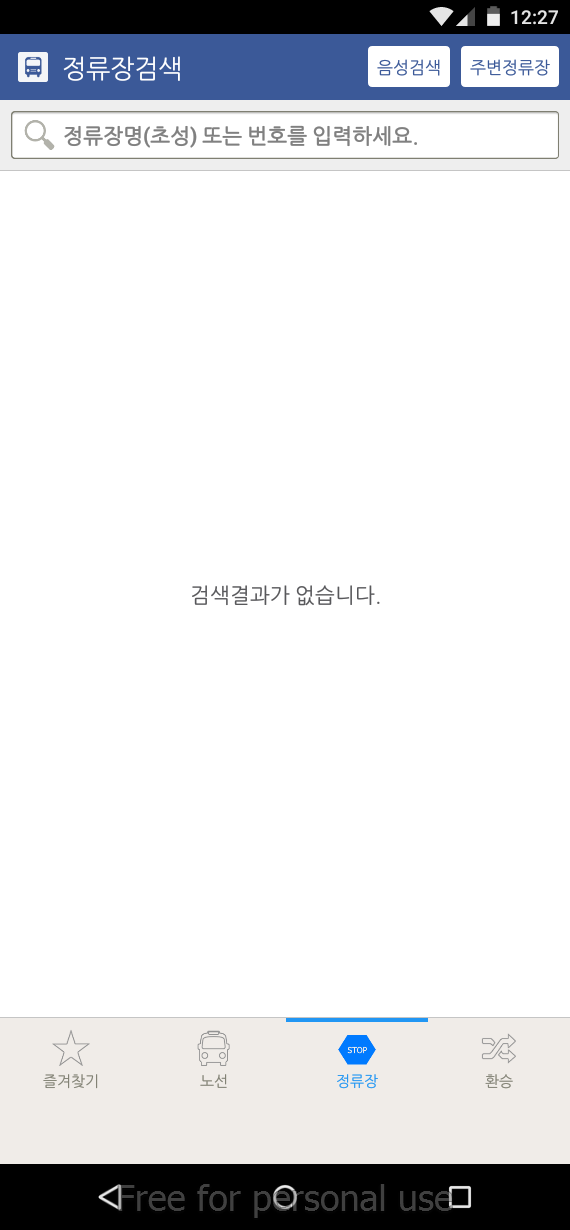
\includegraphics[width=\linewidth]{img/apk_2/screenshots/screenshot-2026-06-26_18.27.34.308.png}
        \caption{Bus stop search screen showing no results during dynamic analysis \twor}
        \label{fig:genymotion2-1}
    \end{subfigure}
    \hfill
    \begin{subfigure}[t]{0.30\linewidth}
        \centering
        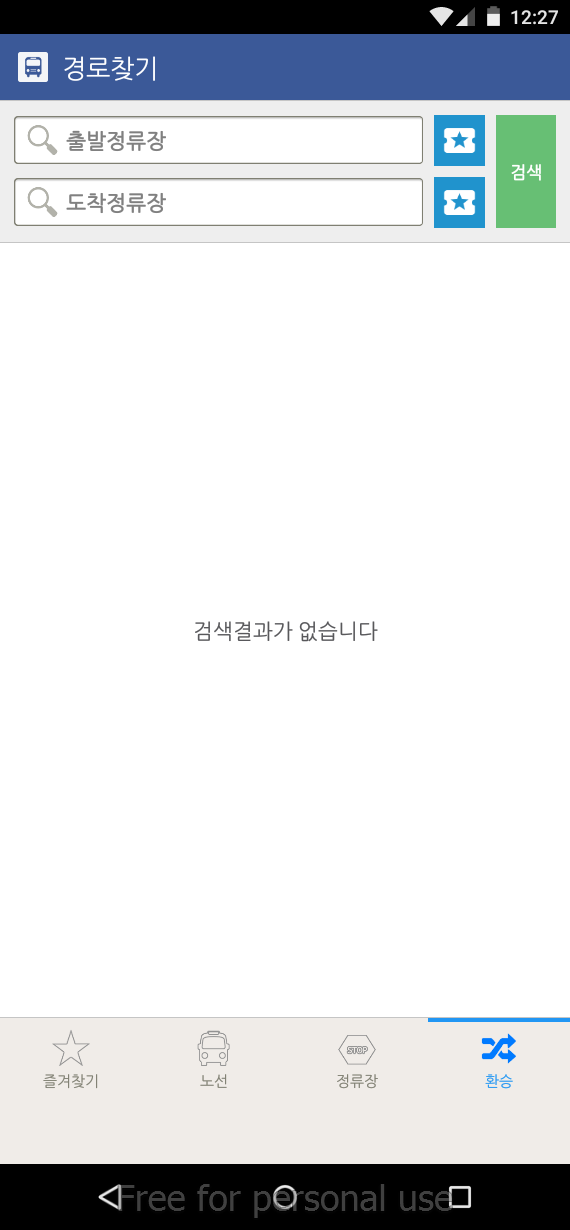
\includegraphics[width=\linewidth]{img/apk_2/screenshots/screenshot-2026-06-26_18.27.37.387.png}
        \caption{Route search screen with departure and arrival fields showing no results \twor}
        \label{fig:genymotion2-2}
    \end{subfigure}
    \hfill
    \begin{subfigure}[t]{0.30\linewidth}
        \centering
        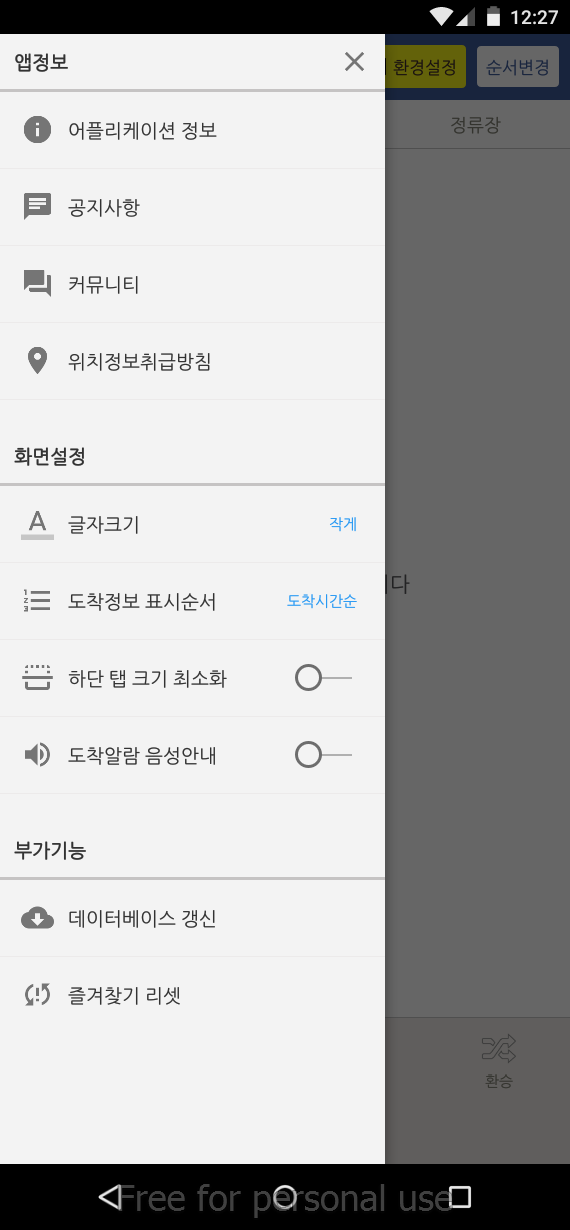
\includegraphics[width=\linewidth]{img/apk_2/screenshots/screenshot-2026-06-26_18.27.42.087.png}
        \caption{App settings menu showing notification and display preferences \twor}
        \label{fig:genymotion2-3}
    \end{subfigure}

    \vspace{0.5cm}

    \begin{subfigure}[t]{0.30\linewidth}
        \centering
        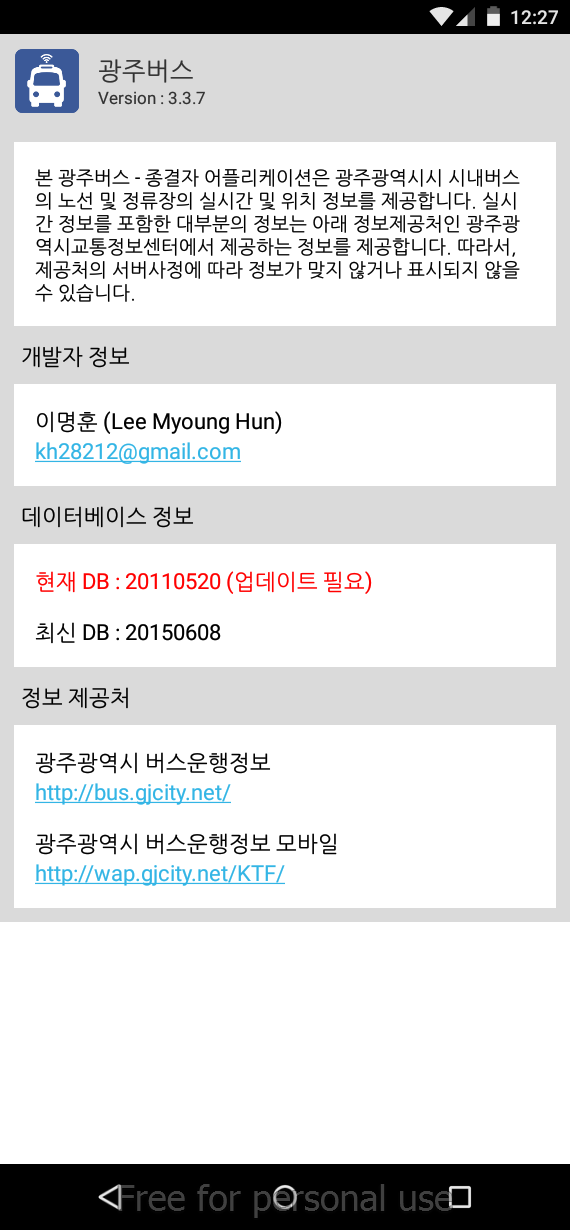
\includegraphics[width=\linewidth]{img/apk_2/screenshots/screenshot-2026-06-26_18.27.51.411.png}
        \caption{App info screen showing outdated database state for \twor}
        \label{fig:genymotion2-4}
    \end{subfigure}
    \hfill
    \begin{subfigure}[t]{0.30\linewidth}
        \centering
        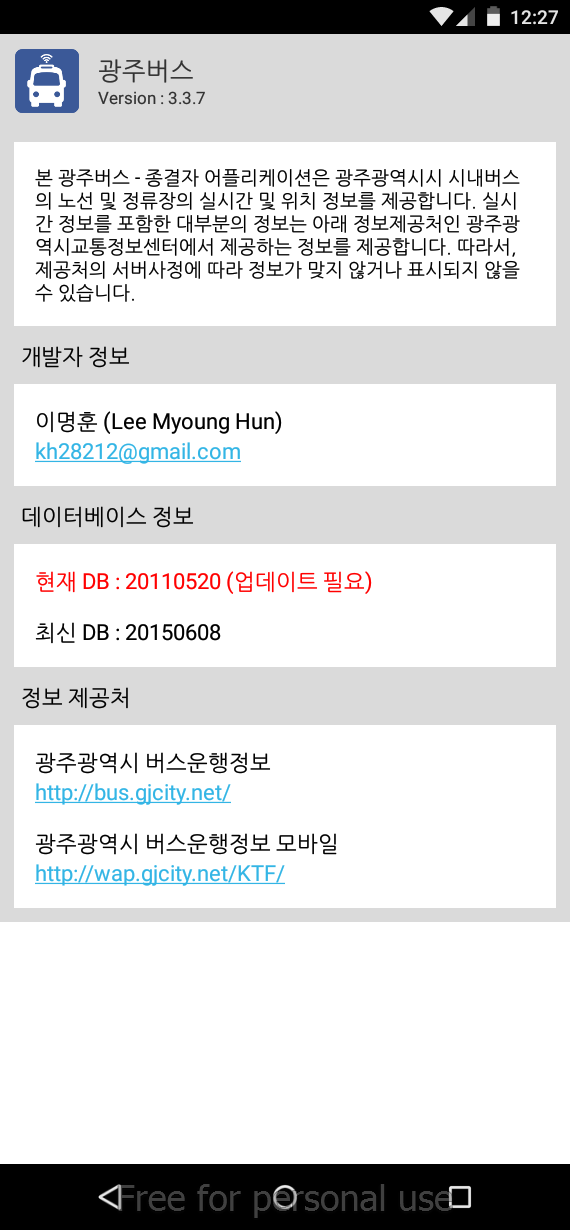
\includegraphics[width=\linewidth]{img/apk_2/screenshots/screenshot-2026-06-26_18.27.51.411.png}
        \caption{Error pop-up indicating database download failure and prompting app restart \twor}
        \label{fig:genymotion2-5}
    \end{subfigure}

    \caption{Genymotion dynamic analysis screenshots of \twor}
    \label{fig:genymotion2-grid}
\end{figure}

\section{Conclusion}

The combined results of VirusTotal, static analysis, MobSF, and Genymotion confirm that \twor\ is malicious and shares the same core dropper architecture identified in \oner.
The structural patterns are consistent across both variants --- native library loading, remote configuration via \texttt{getEnvironmentProperties()}, advertising SDK integration, insecure HTTP communication, and exported components --- confirming family membership.

The defining characteristic of this variant, however, is the measurable evolution of its evasion profile.
Unlike \oner\ , which relies solely on code obfuscation and Java Reflection, \twor\ introduces three additional behavioural tags absent from the previous variant: \texttt{detect-debug-environment}, \texttt{checks-cpu-name}, and \texttt{sets-process-name}.
These indicate that the malware author deliberately hardened this release against dynamic analysis environments --- probing for debuggers, fingerprinting the hardware to detect virtual machines, and manipulating the process name to evade monitoring tools.
This shift from passive obfuscation to active sandbox detection represents a qualitative step in the family's anti-analysis sophistication.

MobSF confirms a high security risk with nine high-severity findings, including Janus vulnerability exposure, SHA-1 signing, StrandHogg weaknesses, and multiple privacy trackers --- a profile identical in count and composition to \oner.
The dynamic analysis in Genymotion further confirms that runtime behaviour is partially driven by remote configuration, consistent with a dropper architecture designed to withhold its payload until the appropriate conditions are met.
The APK should be treated as unsafe: its combination of insecure communication, suspicious permissions, and active anti-analysis evasion demonstrates a clear and deliberate mismatch between its declared purpose and its actual security posture.
